\section{Технологическая часть}

В данном разделе выбирается СУБД, средства реализации приложения,
описаны создание базы данных, триггера, функции и ролей,
а также спроектирован пользовательский интерфейс.

\subsection{Выбор СУБД}

Существует множество различных СУБД, работающих на основе реляционной модели,
каждая из которых имеет свои сильные и слабые стороны.
Среди самых распространенных \cite{most_popular} выделяют MySQL \cite{mysql},
PostgreSQL \cite{postgresql} и SQLite \cite{sqlite}.
Рассмотрим особенности каждой из них.

\begin{enumerate}[label=\arabic*.]
    \item MySQL. Среди достоинств данной СУБД можно выделить высокую
          безопасность и масштабируемость,
          поддержку большей части функционала SQL. Однако, несмотря на
          перечисленные
          положительные аспекты,
          MySQL не сопровождается бесплатной технической поддержкой.
    \item PostgreSQL. В рамках использования этой СУБД имеется возможность
          помимо встроенного SQL использовать различные дополнения,
          отличается поддержкой форматов csv и json, но оперирует большим
          объемом
          ресурсов.
    \item SQLite. Очевидными достоинствами является компактность базы
          данных, которая состоит из одного файла,
          и переносимость.
          Но данная СУБД совершенно не подходит для больших БД, а также не
          поддерживает управление пользователями.
\end{enumerate}

При реализации проекта использован PostgreSQL,
поскольку эта СУБД обладает достаточным набором инструментов для поставленной
задачи.
\subsection{Требования к программе}

Программное обеспечение должно удовлетворять следующим требованиям:
\begin{enumerate}[label=\arabic*.]
    \item возможно подключение к бд;
    \item программа позволяет определять время запросов;
    \item возможно создание программного интерфейса для работы с бд.
\end{enumerate}

\subsection{Средства реализации}

Для реализации ПО был выбран язык программирования Python\cite{python}.

В данном языке есть все требующиеся инструменты для данной курсовой работы.

В качестве среды разработки была выбрана среда VS Code\cite{vscode}, запуск
происходил через команду python back.py.

\subsection{Создание базы данных}

В соответствии с выбранной СУБД и спроектированной базой данных было
осуществлено создание БД и ее сущностей представлено в листинге \ref{dbcreate}.

\begin{lstlisting}[label=dbcreate, caption=Создание БД]
class Visitor(BASE):
    __tablename__ = 'Visitor'
    id = Column(Integer, Identity(always=True), primary_key=True)
    description = Column(Text)
    location = Column(Text)
    view = Column(Text)
    detection = Column(Text)

class Camera(BASE):
    __tablename__ = 'Camera'
    id = Column(Integer, Identity(always=True), primary_key=True)
    location = Column(Text)
    resolution = Column(Text)
    rotation = Column(Text)
    cam_type = Column(Text)
class CameraVisitor(BASE):
    __tablename__ = 'CameraVisitor'
    id_vis = Column(Integer, ForeignKey('Visitor.id'), primary_key=True)
    id_cam = Column(Integer, ForeignKey('Camera.id'), primary_key=True)

class Shelf(BASE):
    __tablename__ = 'Shelf'
    id = Column(Integer, Identity(always=True), primary_key=True)
    location = Column(Text)
    length = Column(Float)
class ShelfVisitor(BASE):
    __tablename__ = 'ShelfVisitor'
    id_shelf = Column(Integer, ForeignKey('Shelf.id'), primary_key=True)
    id_cam = Column(Integer, ForeignKey('Camera.id'), primary_key=True)
class Product(BASE):
    __tablename__ = 'Product'
    id = Column(Integer, Identity(always=True), primary_key=True)
    name = Column(Text)
    location = Column(Text)
    dataEnd = Column(Date)
    weight = Column(Float)
    status = Column(Integer)
    price = Column(Integer)

class ShelfProduct(BASE):
    __tablename__ = 'ShelfProduct'
    id_shelf = Column(Integer, ForeignKey('Shelf.id'), primary_key=True)
    id_product = Column(Integer, ForeignKey('Product.id'), primary_key=True)

class ChainStore(BASE):
    __tablename__ = 'ChainStore'
    id = Column(Integer, Identity(always=True), primary_key=True)
    name = Column(Text)
    location = Column(Text)
    nameDir = Column(Text)
    income = Column(Float)
    consumption = Column(Float)
\end{lstlisting}

\subsection{Создание триггера}

В предыдущем разделе был спроектирован триггер AFTER.
Код его создания представлен в листинге \ref{trigger_code}

\captionsetup{singlelinecheck = false, justification=raggedright}
\begin{lstlisting}[language=sql, caption=Реализация триггера AFTER, label=trigger_code]
CREATE TRIGGER check_location_trigger
AFTER UPDATE ON "Visitor"
FOR EACH ROW
EXECUTE FUNCTION check_location();
\end{lstlisting}
\captionsetup{singlelinecheck = false, justification=centering}

Для этого триггера была написана соответствующая функция.
Код функции представлен в листинге \ref{trigger_func}.

\captionsetup{singlelinecheck = false, justification=raggedright}
\begin{lstlisting}[language=sql, caption=Реализация функции, label=trigger_func]
CREATE FUNCTION check_location() RETURNS TRIGGER AS $$
BEGIN
    IF NEW.location = '0 0' THEN
    RAISE NOTICE 'New visitor added with location: %', NEW.location;
    Return NEW;
    ELSE
    RETURN NULL;
    END IF;
END;
$$ LANGUAGE plpgsql;
\end{lstlisting}
\captionsetup{singlelinecheck = false, justification=centering}

\subsection{Создание ролей и выделение им прав}

В конструкторском разделе была разработана ролевая модель, в которой выделены
следующие роли:
\begin{enumerate}[label=\arabic*.]
    \item employee --- сотрудник;
    \item security --- охрана;
    \item administrator --- администратор.
\end{enumerate}

Соответствующий этой ролевой модели сценарий создания ролей и выделения им прав
представлен на листинге \ref{roles}.

\begin{lstlisting}[language=sql, caption=Создание ролей и выделение им прав, label=roles]
CREATE ROLE employee LOGIN PASSWORD 'postgres';
GRANT SELECT ON TABLE "Visitor" TO employee;

CREATE ROLE security LOGIN PASSWORD 'postgres';
GRANT SELECT ON TABLE "Visitor", "Product", "Shelf" TO security;

CREATE ROLE administrator LOGIN PASSWORD 'postgres';
GRANT ALL PRIVILEGES ON ALL TABLES IN SCHEMA public TO administrator;

\end{lstlisting}
\captionsetup{singlelinecheck = false, justification=centering}

\subsection{Интерфейс программы}

Для работы с БД был разработан интерфейс взаимодействия в виде API \cite{API}.
Для реализации API была использована библиотека fastapi \cite{fastapi}.

В программного интерфейсе реализованы методы: добавления, чтения, обновления и
удаления для каждой таблицы.
Методы представлены на рисунке \ref{fig:api}.

Для использования чтения необходимо указать количество элементов, которые будут
выведены.
Чтобы добавить элемент в таблицу необходимо указать, необходимые поля в
таблице.
Для обновления и удаления элемента таблицы, необходимо указать его номер.

\begin{figure}[ht!]
    \centering
    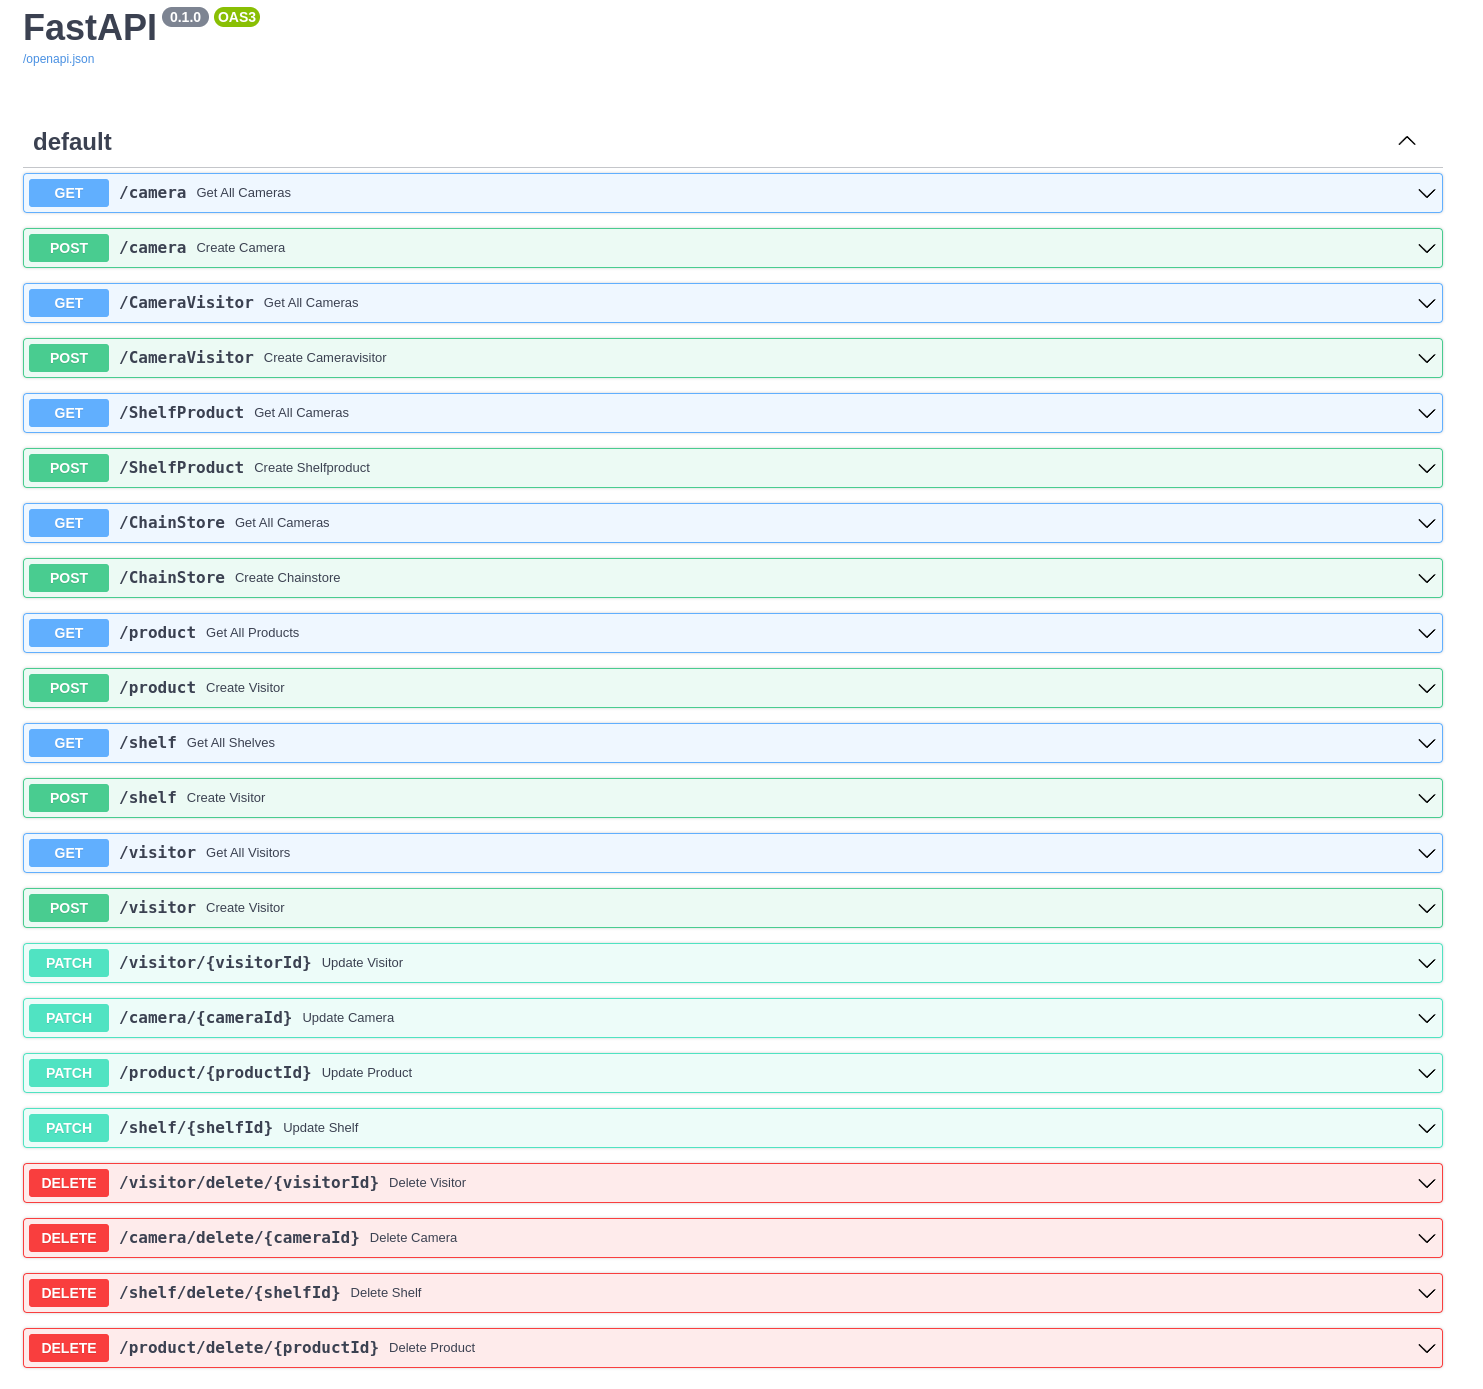
\includegraphics[width=1\linewidth]{assets/images/api.png}
    \caption{Программный интерфейс}
    \label{fig:api}
\end{figure}
\FloatBarrier

\subsection*{Вывод}

В данном разделе выбраны СУБД и средств реализации, описано создание БД,
триггера, ролей с выделением прав.
Также представлен пользовательский интерфейс.